\section{Жорданова нормальная форма линейного оператора}

\begin{reminder}
    Жордановой клеткой, относящейся к  $\lambda \in F$, называется следующая матрица:
    \[J_{k}(\lambda) = \begin{pmatrix}
	\lambda      & 1      & 0      & \dots  & 0\\
		0      & \lambda      & 1      & \dots  & 0\\
		\vdots & \vdots & \vdots & \ddots & \vdots \\
        0      & 0      & \dots      & \lambda  & 1\\
        0      & 0      & 0      & \dots  & \lambda \\
	\end{pmatrix}\]
\end{reminder}

\begin{definition}
    Жордановой матрицей называется блочно-диагональная матрица, по главной диагонали которой идут 
    Жордановы клетки, а остальное заполнено нулями:
    \[J_{k}(\lambda) = \begin{pmatrix}
        J_{k_1}(\lambda_1)      & \dots      & 0    & 0 \\
        \vdots      & J_{k_2}(\lambda_2)      & \dots   & 0 \\
        0   & \vdots     & \ddots    & \vdots \\
        0      & 0      & \dots    & J_{k_n}(\lambda_n) \\
        \end{pmatrix}\]
\end{definition}

\begin{theorem}[Камиль Жордан]
    Пусть $\phi : V \to V$, $\chi_{\phi}$ раскладывается на линейные множители над $F$. 
    Тогда В $V$ существует базис (Жордановый базис), в котором $\phi$ имеет Жорданову матрицу.
\end{theorem}

\begin{note}
    Жроданова матрица определена с точностью до перестановки Жордановых клеток, поэтому базис не единственен в общем случае.
\end{note}

\begin{proof}
    На предыдущих лекциях было доказано:
    \begin{enumerate}
        \item $V = V^{\lambda_1} \oplus V^{\lambda_2} \oplus \dots V^{\lambda_k}$ (подпространства инвариантны), где $\lambda_1, \dots, \lambda_k$ -- все попарно различные собственные значения оператора $\phi$. Тогда в базисе согласованном с таким разложением матрица имеет вид:
         \[A = \begin{pmatrix}
            A_1      & \dots      & 0    & 0 \\
            \vdots      & A_2      & \dots   & 0 \\
            0   & \vdots     & \ddots    & \vdots \\
            0      & 0      & \dots    & A_k \\
            \end{pmatrix}\]
        \item Было доказано, что для $V^{\lambda_i}$ оператор $\phi_{\lambda_i} = \phi - \lambda_i E$ нильпотентен, а значит V 
        раскладывается в сумму циклических подпространств: $V^{\lambda_i} = \displaystyle\sum_{j = 1}^{geom(\lambda_i)} V_{ij}$.
    \end{enumerate}
    Пусть $\dim V_{ij} = k$. Покажем, что на $V_{ij}$ оператор $\phi$ в подходящем базисе имеет вид $J_k(\lambda_i)$:\\ 
    Пусть $k$ - индекс нильпотентности $\phi_{\lambda_i}$ на $V_{ij}$, пусть $x$ - корневой вектор максимальной высоты $k$.\\
    Рассмотрим базис $\langle \phi_{\lambda_i}^{k-1} x, \phi_{\lambda_i}^{k-2} x, \dots, \phi_{\lambda_i}^{1} x \rangle$. 
    Обозначим базисные вектора за $f_{ij}$ следующим образом:
    \begin{gather*}
        f_{i1} = \phi_{\lambda_i}^{k - 1},\\
        f_{i2} = \phi_{\lambda_i}^{k - 2},\\
        \dots
    \end{gather*}
    Подействуем на базис оператором $\phi_{\lambda_i}$. Под действием этого оператора каждый базисный 
    вектор перейдет в предыдущий (первый перейдет в $0$): $\phi_{\lambda_i}(f_{i1}) = \overline{0}, \dots, \phi_{\lambda_i}(f_{ik}) = f_{i(k - 1)}$. 
    Тогда матрица оператора $\phi_{\lambda_i}$ будет иметь в базисе $f$ вид $J_k(0)$.
    Тогда $\phi \vert_{V_{ij}} = \lambda_1 \epsilon + J_k(0) = J_k(\lambda_i)$
    Мы доказали, что в подходящем базисе сужение на подпространство имеет вид Жордановой клетки. Тогда из
    $V = \displaystyle\sum_{i = 1}^{k} \displaystyle\sum_{j = 1}^{geom(\lambda_i)} V_{ij}$
    вытекает, что матрица оператора в подходящем базисе (Жордановом базисе) имеет вид Жордановой матрицы.
\end{proof}

\begin{corollary}
    Если $V$ - линейное пространство над полем комплексных чисел, то всякий оператор в таком пространстве имеет Жорданову нормальную форму.
\end{corollary}

\subsection{Жорданова диаграмма}

\begin{definition}
    ЖД соотв ЖМ $J$ называется набор точек на плоскости, в котором точка с координатой $(i, j)$ 
    изображает вектор $f_{ij}$ ЖБ. Под каждым столбцом ЖД указывается соответствующее векторам этого 
    столбца собственные значения.
\end{definition}

\begin{example}
    Пусть $\phi$ имеет в некотором базисе следующую матрицу -- 
        \[A = \begin{pmatrix}
        \lambda & 1        & 0       & 0       & 0        & 0    &0    & 0\\
        0       & \lambda  & 1       & 0       & 0        & 0    &0    & 0\\
        0       & 0        & \lambda & 0       & 0        & 0    &0    & 0\\
        0       & 0        & 0       & \lambda & 1        & 0    &0    & 0\\
        0       & 0        & 0       & 0       & \lambda  & 0    &0    & 0\\
        0       & 0        & 0       & 0       & 0        & \mu  &1    & 0\\
        0       & 0        & 0       & 0       & 0        & 0    &\mu  & 0\\
        0       & 0        & 0       & 0       & 0        & 0    &0    & \nu
        \end{pmatrix}\]
    Четыре Жордановы клетки: порядков $2$ и $3$ с собственным значением $\lambda$, порядка $2$ с собственным значением $\mu$ и порядка $1$ с собственным значением $\nu$. \\ Такая матрица является Жордановой. Начнем выписывать Жорданов базис: $f_{11}, f_{12}, f_{13}, f_{21}, f_{22}, f_{31}, f_{32}, f_{41}$.
    В общем случае если мы пишем Жорданов базис в виде $f_{ij}$, коэффициенты означают номер клетки и 
    номер вектора относительно данной клетки соответственно. Теперь вектор $f_{ij}$ можно сопоставить 
    точке на графике с координатами $(i, j)$. Если под каждым столбцом указать соответствующие векторам столбца собственные значения, то полученный график называется Жордановой диаграммой.
    \begin{center}
        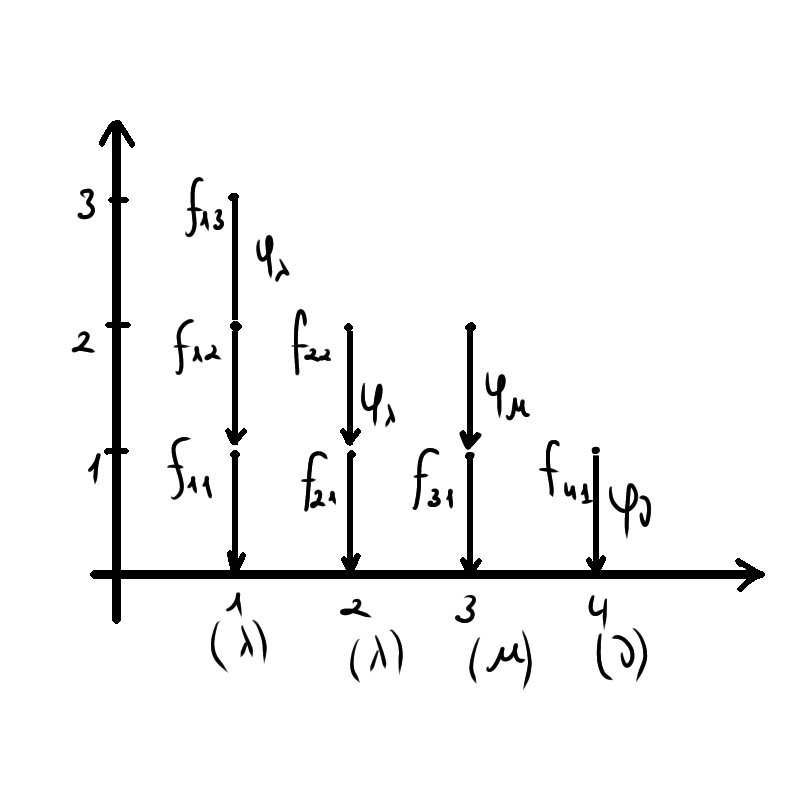
\includegraphics[width = 0.4\textwidth]{images/lec6_1.PNG}
    \end{center}
\end{example}

\begin{note}
    Столбцы не обязательно должны быть отсортированы в порядке невозрастания, диаграмма соответствует 
    конкретной матрице и меняется при перестановке клеток местами.
\end{note}

\begin{proposition}[Свойства Жордановой диаграммы]~
    \begin{enumerate}
        \item Соответствие Жордановой матрицы $J$ и Жордановой диаграммы $J$ взаимно однозначно.
        \item Векторы Жордановой диаграммы, относящиеся к собственному значению $\lambda_i$, образуют базис 
        в корневом подпространстве $V^{\lambda_i}$.
        \item Если вектор $f_{ij}$ относится к собственному значению $\lambda_i$, 
        то он является корневым вектором, относящимся к $\lambda_i$ высоты $j$, 
        то есть $\phi_{\lambda_i}^j f_{ij} = \overline{0}$, но $\phi_{\lambda_i}^{j-1} f_{ij} \neq \overline{0}$.
        На высоте 1 в Жордановой диаграммы находятся собственные векторы оператора $\phi$.
        \item Если $f_{ij}$ относится к собственному значению $\lambda_{j}$, то $\phi_{\lambda_i} f_{ij} = f_{i(j-1)}$.
        %Нарисовать диаграмму со стрелочками вниз и нули на нижней линии.
        \item Каждый столбец в Жордановой диаграмме является изображением циклического подпространства для оператора $\phi_{\lambda_i}$. Общее число столбцов в Жордановой диаграмме $\displaystyle\sum_{i=1}^{k} geom(\lambda_i)$.
    \end{enumerate}
\end{proposition}

\subsection{Построение Жордановой диаграммы линейного оператора}

\begin{proposition}
    Пусть $\phi : V \to V$. Тогда справедливы следующие вложения:
    \begin{enumerate}
        \item $\ker \phi^0 \subseteq \ker \phi \subseteq \ker \phi^2 \subseteq \dots$
        \item $\im \phi^0 \supseteq \im \phi \supseteq \im^2 \supseteq \dots$
    \end{enumerate}
    Причем обе цепочки стабилизируются за конечное число шагов.
\end{proposition}

\begin{proof}
    Индукция по $n \in \Z_{\geq 0}$:

    \begin{enumerate}
        \item База индукции: $\ker \phi^0 = \ker E = {\overline{0}} \subseteq \ker \phi \; \forall \phi$ и аналогично $\im \phi^0 = \im E = V \supseteq \im \phi \forall \phi$.
        \item Докажем, что $\ker \phi^n \subseteq \ker \phi^{n+1}$ (где $n \in \N$):
        
        Если $x \in \ker \phi^n$, тогда $\phi^n x = 0$ и $\phi ^{n + 1} x = \phi (\phi ^ n x) = \phi (\overline{0}) = \overline{0}$. \\
        Докажем теперь аналогичное вложение для образов: пусть $y \in \im \phi^{n + 1}$, тогда существует $x$, такой что $y = \phi^{n + 1} x = \phi^n(\phi(x)) = \phi^n z \in \im \phi^n$. Следовательно, $\im \phi^{n + 1} \subseteq \im \phi^n$.
    \end{enumerate}
\end{proof}

\begin{algorithm}[Построение Жордановой диаграммы]

Покажем, как это использовать для нахождения Жордановой матрицы. Обозначим размерности ядер за $n_i$ соответственно: $\dim \ker \phi^i = n_i$. Выпишем для одного подпространства $U_{\lambda}$ все вложенные в него:
\begin{eqnarray}  
    \{0\} \subseteq \ker \phi_{\lambda} = \langle f_{11}, f_{12}\rangle \subseteq \ker \phi_{\lambda}^2 
    = \langle f_{11}, f_{21}, f_{12}, f_{22} \rangle \subseteq \ker \phi_{\lambda}^3 = 
    \langle f_{11}, f_{21}, f_{12}, f_{22}, f_{13} \rangle, \\ (n_1 = 2, n_2 = 4, n_3 = 5).
\end{eqnarray}
Тогда число точек в Жордановой диаграмме на высоте $j$ равно $d_j = n_j - n_{j-1}$, откуда для нашего примера соответствующие $d$ равны $d_1 = 2-0=2, d_2 = 4-2=2, d_3 = 5-4=1$.

Если в корневом пространстве $V^{\lambda}$ ввести обозначения $d_j$ - число векторов (точек) на высоте $j$, то $d_j = n_j - n_{j-1}$, где $n_0 = 0$, $n_k = \dim \ker (\phi - \lambda_i E)^k$.
Это работает, потому что при применении оператора $j$ раз обнулятся все векторы на высоте не выше $j$, 
тогда при применении на $1$ раз меньше обнулятся все, кто ниже, искомое количество - те, кто обнуляется при применении $j$ раз и не обнуляется при применении на 1 раз меньше.

Строим ядра (и образы) до тех пор, пока они не стабилизируются (будут равны).
\end{algorithm}

\begin{agreement}
    При построении будем упорядочивать столбцы по невозрастанию.
\end{agreement}

\begin{note}
    Описание ядер $\phi_{\lambda_i}^k$ и вычисление их размерностей можно производить в любом базисе.
\end{note}

\begin{theorem}[]
    Жорданова нормальная форма линейного оператора $\phi$ опеределена однозначно с точностью до перестановки Жордановых клеток, стоящих на главной диагонали. 
    Утверждение складывается из двух промежуточных:
    \begin{enumerate}
        \item Сумма порядков клеток, относящихся к собственному значению $\lambda_i$, не зависит от выбора Жорданова базиса.
        \item Для оператора $\phi$, имеющего единственное собственное значение, порядки Жордановых клеток определяются однозначно.
    \end{enumerate}
\end{theorem}

\begin{proof}~
    \begin{enumerate}
        \item  Зафиксируем Жорданов базис и корневое подпространство $V^{\lambda_i}$ и выберем все векторы Жорданова базиса, относящиеся к $\lambda_i$. Обозначим $V(\lambda_i) = \langle f_{ij} | f_{ij}$ относящиеся к $\lambda_i \rangle$. \\
        Пусть $l_i$ - максимальный порядок Жордановых клеток Жордановой матрицы, отвечающих $\lambda_i$, $(J_k(\lambda_i) - \lambda_i \epsilon)^{l_i} = 0$. 
        Оператор нильпотентен и за несколько его применений все векторы базиса обратятся в 0.
        Таким образом $(\phi - \lambda_i \epsilon)^{l_i} \vert_{V(\lambda_i)} = 0$.
        $\forall i V(\lambda_i) \subseteq V^{\lambda_i}$ -- так как все векторы аннулируются.
        \begin{enumerate}
            \item $V = V^{\lambda_1} \oplus V^{\lambda_2} \dots \oplus V^{\lambda_k}$
            \item $V = V(\lambda_1) \oplus V(\lambda_2) \dots \oplus V(\lambda_k)$.
        \end{enumerate}
        По теореме о характеризации прямой суммы второе выражение является прямой суммой, а значит верны вложения и в обратную сторону(из соображений размерности).
        \item Пусть единственное собственное значение -- 0. Покажем, что размеры клеток в Жордановой нормальной форме определены однозначно. 
        Как было доказано на предыдущих лекциях, из того, что оператор нильпотентен, существует разложение в прямую сумму циклических подпространств.
        \begin{center}
            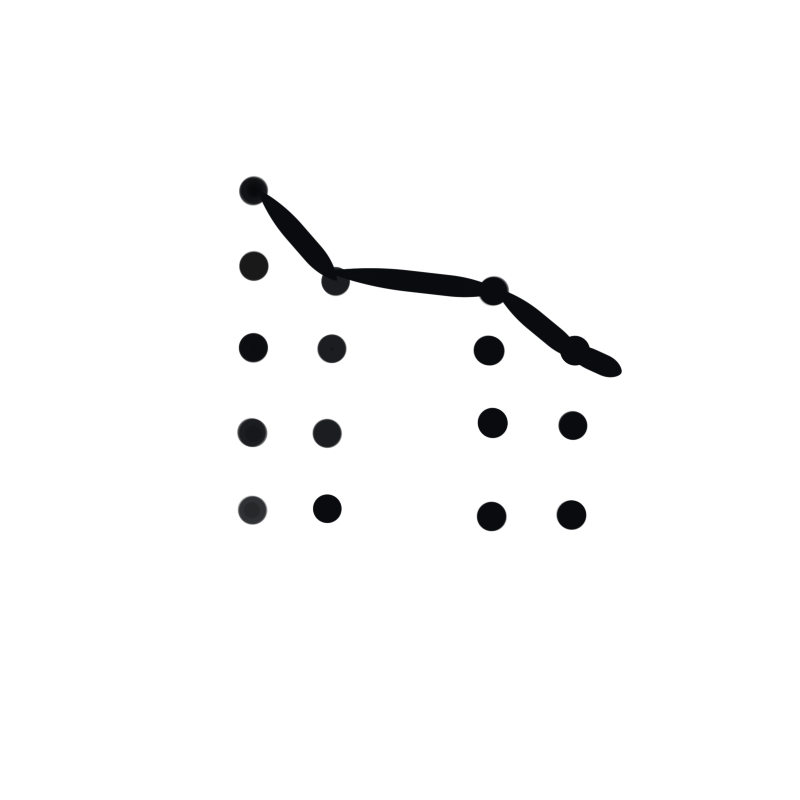
\includegraphics[width = 0.2\textwidth]{images/lec6_5.PNG}
        \end{center}
        Длины строк определены однозначно: $d_j = n_j - n_{j-1}$, $n_j = \dim ker \phi^j$. Таким образом порядок клеток тоже можно определить однозначно.
    \end{enumerate}
\end{proof}

\subsubsection{Эффективный способ построения Жорданова базиса}

\begin{lemma}[О восстановленных циклических цепочках]~
    Пусть $\phi$ - линейно факторизуемый оператор в $V$, 
    $z_1$, $z_2$, $\dots$ $z_n$ -- линейно независимая система собственных векторов оператора $\phi$, относящихся к $\lambda$ (собственное значение), $x_i$ имеет высоту $l_i$.
    Пусть $\langle \phi_{\lambda}^{l_i-1} x_i, \phi_{\lambda_i}^{l_i-2} x_i, \dots, \phi_{\lambda}^{1} x_i, x_i \rangle$ -- циклическая целочисленная цепочка, такая что $\phi_{\lambda}^{l_i - 1} x_i = z_i$. Тогда $\bigcup\limits_{i = 1}^n (\phi_{\lambda}^{l_i - 1} x_i \dots \phi_{\lambda} x_i, x_i)$ -- тоже линейно независимая система.
\end{lemma}

\begin{proof}
    Пусть полученная система линейно зависима. Тогда сумма $\displaystyle\sum_{i} \displaystyle\sum_{j} \alpha_{ij} f_{ij} = \overline{0}$ -- нетривиальная линейная комбинация.
    Пусть $f_{ij} = \phi_{\lambda}^{l_i - j}$ имеет высоту $j$, тогда $\phi_{\lambda}^j(f_{ij}) = \phi_{\lambda}^{l_i} x_i = \overline{0}$, причем  $\phi_{\lambda}^{j - 1}(f_{ij}) = \phi_{\lambda}^{l_i - 1} x_i \neq \overline{0}$.
    \begin{center}
        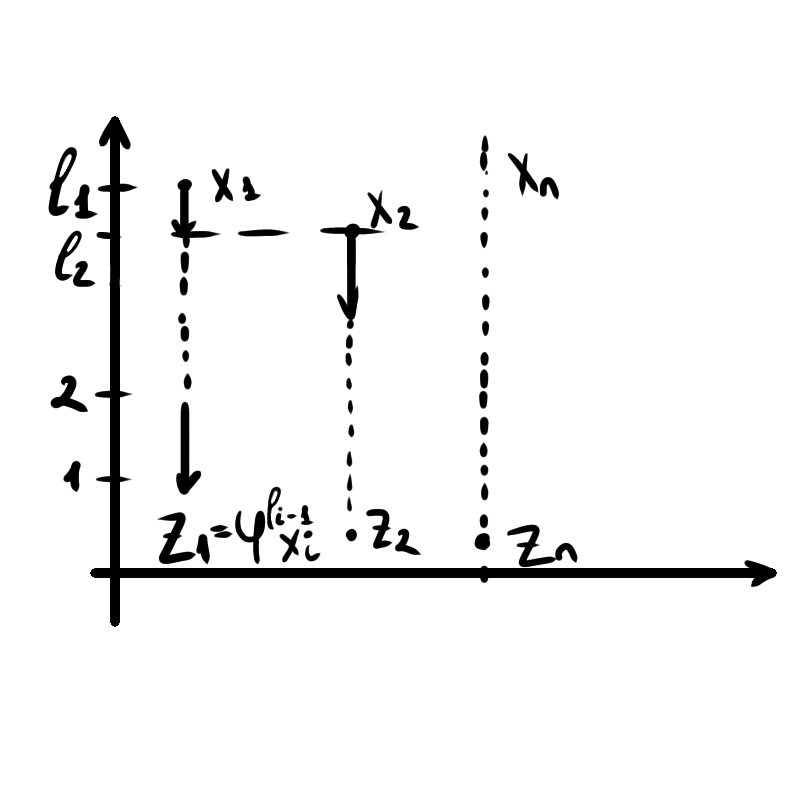
\includegraphics[width = 0.45\textwidth]{images/lec6_2.PNG}
    \end{center}
    Пусть $\alpha_{it}$ - ненулевой коэффициент с наибольшим вторым индексом. Подейтсвуем $\phi_{\lambda}^{t-1}$ на сумму по $i, j$.
    Тогда: $$\phi_{\lambda}^{t-1} (\alpha_{it} f_{it}) = \alpha_{it} \phi_{\lambda}^{t-1} \phi_{\lambda}^{l_i - t} x_i 
    = \alpha_{it} \phi_{\lambda}^{l_i - 1}x_i = \alpha_{it} z_i.$$ Таким образом,для всех коэффициентов верно $\displaystyle\sum_{i = 1}^n \alpha_{it}z_i = \overline{0}, \alpha_{it} \neq 0$, что приводит к противоречию с линейной зависимостью системы векторов $z_1, \dots z_n$.
\end{proof}

\begin{algorithm}[Построение Жорданова базиса]~

Будем строить Жорданов базис отдельно для каждого корневого подпространаства $V^{\lambda}$, и пусть высоты циклических подпространств идут в порядке невозрастания, наибольшая высота равна $l$ ($\dim V^{\lambda} = d$) и пусть таких цепочек $n$ штук, следующая высота $p$ и таких цепочек $m$. \\
    \begin{center}
        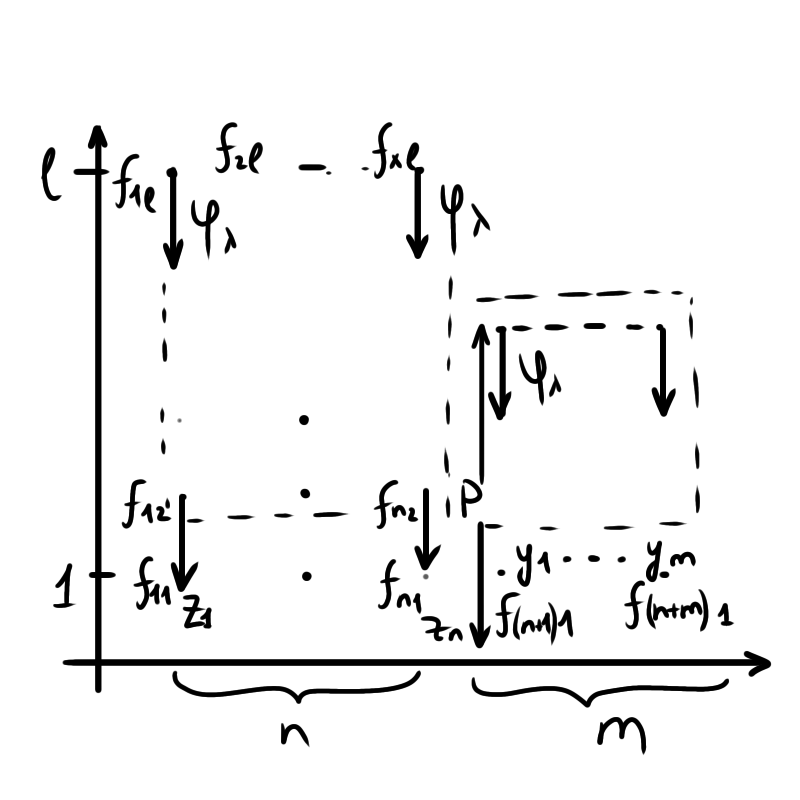
\includegraphics[width = 0.5\textwidth]{images/lec6_4.PNG}
    \end{center}
Пусть $z_1, \dots, z_n$ -- линейно независимая система собственных векторов. Восстановлены циклические цепочки $f_{i1}, \dots f_{il}, 1 \leq i \leq n$. Причем $\ker \phi_{\lambda} = \{ f_{11} \dots f_{n1} \dots \}$.
$\dim Im \phi_{\lambda} = d - \dim \ker \phi_{\lambda} = d - n_1$ - все точки диаграммы кроме самых верхних(то же самое: все точки без нижнего слоя).
$\dim \ker \phi_{\lambda}^2 = n_2$, $\dim \im \phi_{\lambda}^2 = d - n_2$ - все точки кроме верхних двух слоев(то же самое: без двух нижних строчек).
Таким образом, на каждом шаге мы снимаем верхний слой (на каждом шаге у нас "тает" слой, совсем как мороженое).
После того как мы сняли все слои кроме последнего, остался слой из собственных векторов:
$\im \phi_{\lambda}^{l-1} = \langle z_1, z_2, \dots, z_n\rangle$.

Рассмотрим циклическую цепочку, порожденную $x_i$:
$$\bigcup\limits_{i = 1}^n (\phi_{\lambda}^{l - 1} x_i \dots \phi_{\lambda} x_i, x_i)$$
Это линейно независимая система векторов в количестве $l \cdot n$. Тогда если $n \cdot l = d$, Жорданов базис построен. Если же $n \cdot l < d$, то строим базис дальше. Теперь пусть есть циклические цепочки меньших высот (высоты $p$). 
Снова рассматриваем образ соответствующий нижнему слою ($\im \phi_{\lambda}^{p -1 }$). 
Однако теперь в него так же попадут векторы из линейной оболочки уже построенной части базиса.\\
$\im \phi_{\lambda}^{p - 1} \supseteq \langle \phi_{\lambda}^{p - 1}(x_i), \phi_{\lambda}^{p - 1}(\phi_{\lambda} x_i), \dots \phi_{\lambda}^{p - 1}(\phi_{\lambda}^{l - p} x_i \rangle$. Дополняем в $\im \phi_{\lambda}^{p -1}$ линейную оболочку до базиса векторами $y_1, \dots y_n$ -- собственные векторы с собственным значением $\lambda$. По $y_1, \dots y_n$ восстанавливаем циклические цепочки и присоединяем к Жорданову базису.
\end{algorithm}

\begin{example}
    Рассмотрим матрицу и найдем для нее Жорданову диаграмму, Жорданову нормальную форму, Жорданов базис:
         \[A = \begin{pmatrix}
        1      & 0     & 0    & 0  & 0 \\
        1      & -1    & 0    & 0  & -1 \\
        1      & -1    & 0    & 0  & -1 \\
        0      & 0    & 0    & 0  & -1 \\
        -1     & 1     & 0    & 0  & 1 \\
        \end{pmatrix}\]

    \begin{enumerate}
        \item Находим характеристический многочлен как определитель: 
        $\chi_{\phi}(\lambda) = \det (A - \lambda E) = \lambda^4 (1 - \lambda)$. (можно посчитать по теореме Лапласса относительно 3 и 4 столбцов)
        Тогда собственные значения $\lambda_1 = 0$, $alg(0) = 4$, $\lambda_2 = 1$, $alg(1) = 1$ (так как была теорема о том, что $geom(\lambda) \leq alg(\lambda)$, но при этом хотя бы $1$, то $geom(1) = 1$). 
        Пространство представляется в виде $V = V^0 + V^1$
        \item Для всех собственных значений $\lambda$:
        $\{0\} \subseteq \ker \phi \subseteq \phi^2 \dots$ \\
        Ищем ранг матрицы $A$: $\dim \im \phi = rk A$, $rk A = 3$, $n_1 = \dim \ker \phi = 5 - 3 = 2$.
        Находим матрицу для $\phi^2$ возводя $A$ в квадрат.
         \[A^2 = \begin{pmatrix}
        1      & 0     & 0    & 0  & 0 \\
        1      & 0     & 0    & 0  & 0 \\
        1      & 0     & 0    & 0  & 0 \\
         1      & -1    & 0    & 0  & -1 \\
        -1     & 0     & 0    & 0  & 0 \\
        \end{pmatrix}\]
        $rg A^2 = 3$, $n_2 = \dim \ker \phi^2 = 5 - 2 = 3$.
        Стабилизации не произошло, поэтому вычисляем $A^3$.
         \[A^3 = \begin{pmatrix}
        1      & 0     & 0    & 0  & 0 \\
        1      & 0     & 0    & 0  & 0 \\
        1      & 0     & 0    & 0  & 0 \\
         1      & 0     & 0    & 0  & 0 \\
        -1     & 0     & 0    & 0  & 0 \\
        \end{pmatrix}\]
        Заметим, что при умножении первый столбец не изменился, 
        а значит нам повезло, и он является собственным вектором для $\lambda = 1$.
        Полученная матрица состоит только из первого столбца, остальные значения - нули, 
        при этом первый столбец сохраняется при умножении на $A$, а значит $A^3 = A^4 = A^5 = \dots$, $rk A^3 = 1 = rk A^4 = \dots$, стабилизация произошла. ($n_3 = \dim \ker \phi^3 = 5 - 1 = 4$)
        \item Жорданова диаграмма имеет вид:
        \begin{center}
            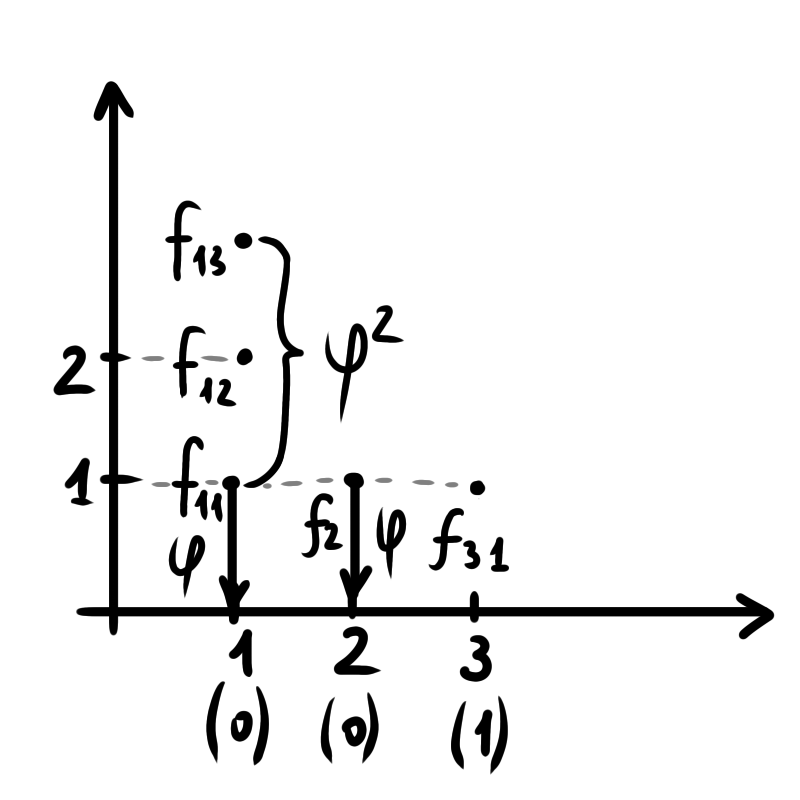
\includegraphics[width = 0.35\textwidth]{images/lec6_3.PNG}
        \end{center}
        \begin{eqnarray}
            d_1 = n_1 - 0 = 2   \\
            d_2 = n_2 - n_1 = 1 \\
            d_3 = n_3 - n_2 = 1 \\
            d_4 = d_5 = \dots = 0
        \end{eqnarray}
        \item Жорданова нормальная форма имеет вид:
         \[J = \begin{pmatrix}
        0      & 1     & 0    & 0  & 0 \\
        0      & 0     & 1    & 0  & 0 \\
        0      & 0     & 0    & 0  & 0 \\
         0      & 0     & 0    & 0  & 0 \\
        0     & 0     & 0    & 0  & 1 \\
        \end{pmatrix}\]
        Матрица состоит из трех Жордановых клеток: размера $3$ (с собственным значением $0$), размера $1$(с собственным значением $0$), размера $1$(с собственным значением $1$).\\
        Теперь подберем базис, соответствующий этой матрице: для выбора векторов, выберем сначала первые:
        $\langle f_{12}, f_{21}\rangle = \langle e_3, e_4\rangle$
        $Im \phi^2 = \langle (1, 1, 1, 1, -1)^T, (0, 0, 0, 1, 0)^T \rangle$. 
        Тогда так как $e_3$ не лежит в образе, а $e_4$ лежит, то они соответствуют векторам: $f_{11} = e_4 = (0, 0, 0, 1, 0)^T$, $f_{21} = (0, 0, 1, 0, 0)^T$. Как мы уже выяснили $f_{31} = (1, 1, 1, 1, -1)^T$. Тогда пусть $f_{13} = e_2 = (0, -1, 0, 0, 0)^T$ и $f_{12} = (0, 1, 1, 0, -1)^T$.
        \item Теперь можно сказать, что Жорданов базис равен $(f_{11}, f_{12}, f_{13}, f_{21}, f_{31})$. 
        Типичная ошибка - выписывать векторы из диаграммы сверху вниз, а не снизу вверх.
    \end{enumerate}
\end{example}

\begin{exercise}
    Найти матрицу перехода от $A$ и $J$ как $S^{-1}AS = J$.
\end{exercise}